\documentclass[11pt,compress,t,notes=noshow, aspectratio=169, xcolor=table]{beamer}

\usepackage{../../style/lmu-lecture}
% Defines macros and environments
% This file is included in slides and exercises

% Rarely used fontstyle for R packages, used only in 
% - forests/slides-forests-benchmark.tex
% - exercises/single-exercises/methods_l_1.Rnw
% - slides/cart/attic/slides_extra_trees.Rnw
\newcommand{\pkg}[1]{{\fontseries{b}\selectfont #1}}

% Spacing helpers, used often (mostly in exercises for \dlz)
\newcommand{\lz}{\vspace{0.5cm}} % vertical space (used often in slides)
\newcommand{\dlz}{\vspace{1cm}}  % double vertical space (used often in exercises, never in slides)
\newcommand{\oneliner}[1] % Oneliner for important statements, used e.g. in iml, algods
{\begin{block}{}\begin{center}\begin{Large}#1\end{Large}\end{center}\end{block}}

% Don't know if this is used or needed, remove?
% textcolor that works in mathmode
% https://tex.stackexchange.com/a/261480
% Used e.g. in forests/slides-forests-bagging.tex
% [...] \textcolor{blue}{\tfrac{1}{M}\sum^M_{m} [...]
% \makeatletter
% \renewcommand*{\@textcolor}[3]{%
%   \protect\leavevmode
%   \begingroup
%     \color#1{#2}#3%
%   \endgroup
% }
% \makeatother


\title{Interpretable Machine Learning}
% \author{LMU}
%\institute{\href{https://compstat-lmu.github.io/lecture_iml/}{compstat-lmu.github.io/lecture\_iml}}
\date{}

\begin{document}

	
% Set style/preamble.Rnw as parent.

% Load all R packages and set up knitr

% This file loads R packages, configures knitr options and sets preamble.Rnw as 
% parent file
% IF YOU MODIFY THIS, PLZ ALSO MODIFY setup.Rmd ACCORDINGLY...

% Defines macros and environments

 \newcommand{\titlefigure}{figure/counterfactuals_obj}
\newcommand{\learninggoals}{
\item Understand the motivation behind CEs
\item See the mathematical foundation of CEs}

\lecturechapter{Counterfactual Explanations}
\lecture{Interpretable Machine Learning}

% ------------------------------------------------------------------------------

\begin{vbframe}{Counterfactual Explanations}
	\begin{itemize}
	    \item \textbf{Counterfactual explanations} (CEs) or short \textbf{counterfactuals} explain particular decisions of an ML model by presenting an alternative input whose prediction equals a desired outcome.
		\item CEs represent \textbf{close neighbors} of a data point we are interested in, but belonging to the \textbf{desired outcome class}. 
		\item Therefore, CEs reveal what minimal changes to the input are sufficient to receive a different response.\\
		$\rightarrow$ Very useful if there is a chance to change the input features (e.g., by changing behaviour).
		\item Due to their natural interpretation, the targeted audience of CEs are often end-users not ML engineers.
%		\item While we focus here exclusively on their application to tabular data, they can also be applied to image and text data. 
	\end{itemize}
\end{vbframe}

\begin{vbframe}[allowframebreaks]{Example: Credit Risk Application} 
	\begin{itemize}
		\item $\textbf{x}$: customer and credit information
		\item $y$: grant or reject credit
	\end{itemize}
	\begin{center}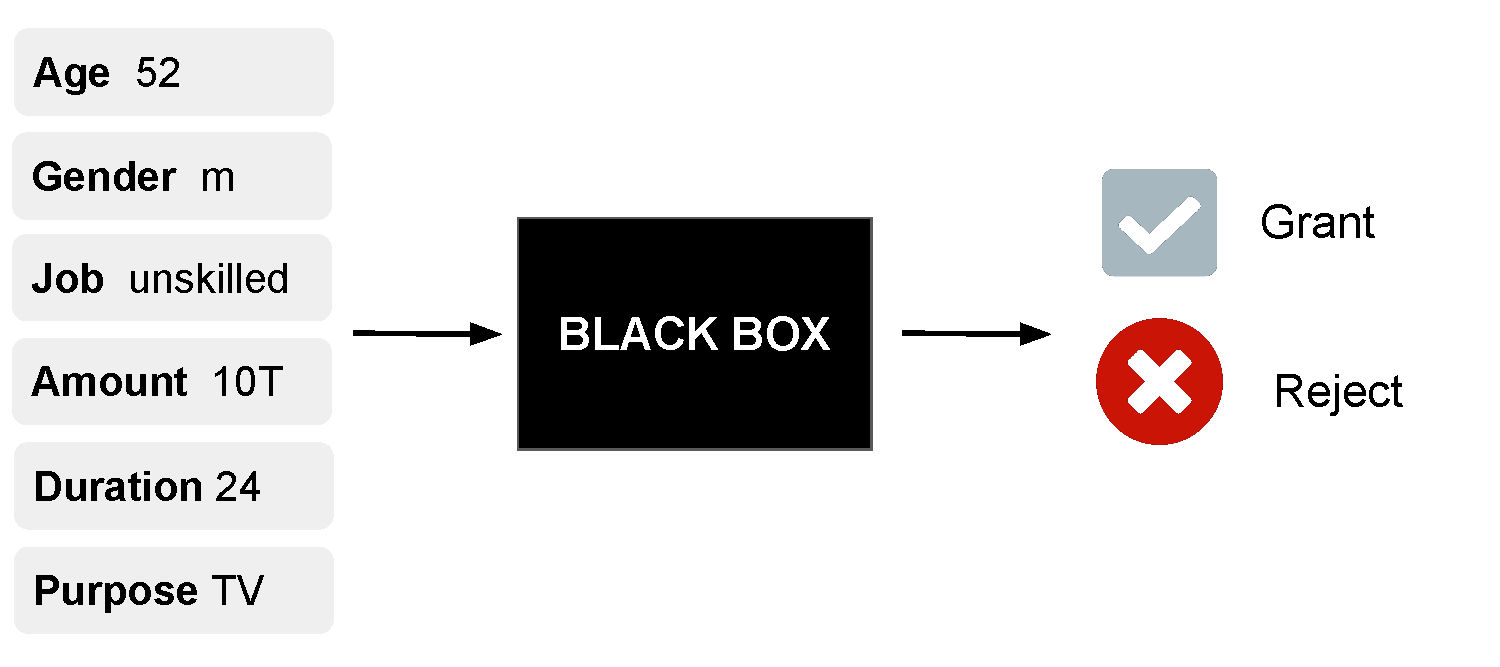
\includegraphics[width=0.6\linewidth, page=1]{figure/counterfactuals_credit.pdf} \end{center}
	
	Questions: 
	\begin{itemize}
		\item Why was the credit rejected? 
		\item Is it a fair decision? 
		\item How should $\xv$ be changed so that the credit is accepted?  
	\end{itemize}
	
	\framebreak
	Counterfactual Explanations provide answers in the form of "What-If"-scenarios. 
	\begin{center}\includegraphics[width=0.6\linewidth, page=2]{figure/counterfactuals_credit.pdf} \end{center}
	
	``If the person was more skilled and the credit amount had been reduced to \$8.000, his credit would have been granted."  \\[0.2cm]
	
%	 \begin{center}\includegraphics[width=1\linewidth, page=3]{figure/counterfactuals_credit.pdf} \end{center}
%	Input: Desired target, original data point, predictor, observed data\\[0.1cm]
%	Output: Data points which minimize  
%	\begin{enumerate}
%		\item Distance of prediction to desired prediction $|\fh(x) - y'|$
%		\item Number of feature changes $\sum_{j = 1}^p I_{x_j \neq x^*_j}$
%		\item Distance to original data point $d(x, x^*)$ (Gower)
%		\item Distance to observed data points $d(x, X^{obs})$
%	\end{enumerate}
	
\end{vbframe}



\begin{vbframe}{Aims \& Roles}
	CEs can serve various purposes, the user can decide what to learn from them. For example:\newline
	``If the person had been one year older and the credit amount had been increased to \$12.000, her credit would have been granted."  \\[0.2cm]
	\begin{itemize}
		\itemsep1.3em
		\item \textbf{Guidance for future actions:} \textit{Ok, I'll apply again next year for the higher amount.}
		\item \textbf{Provide reasons:} \textit{Interesting, I did not know that age plays a role in loan applications.}
		\item \textbf{Provide grounds to contest the decision:} \textit{How dare you, I do not want to be discriminated for my age in an application.}
		\item \textbf{Detect model biases:} \textit{There is a bug, an increase in amount should not increase approval rates.}
	\end{itemize}
\end{vbframe}

\begin{vbframe}{Philosophical Basis}
%Interestingly, counterfactuals have a long-standing tradition in philosophy and, in fact the IML discussion of CEs is based on the work of Lewis (1973). 
Counterfactuals have a long-standing tradition in analytic philosophy. %and, in fact the IML discussion of CEs is based on the work of Lewis (1973). 
Accoding to Lewis (1973), a \textbf{counterfactual conditional} is a statement of the form:	
\begin{equation}
		\textnormal{``If $S$ was the case, $Q$ would have been the case."}
		\label{eq:sent}
\end{equation}
	\begin{itemize}
		\item $S$ must relate to a past event that didn't occur. In that sense counterfactuals run \textbf{contrary} to the \textbf{facts}.
		\item In Lewis's framework Statement~(\ref{eq:sent}) is true, if in all possible worlds most similar to the actual world where $S$ had been the case, $Q$ would have been the case. 
		\item A world is similar to another if laws are maximally preserved between the worlds and only a few facts are changed.
%		\item Lewis's proposal is hotly debated in philosophy, particularly his notion of similarity between worlds remains controversial. 
	\end{itemize}
\end{vbframe}

\begin{vbframe}{Philosophical Basis}
% According to Lewis:\newline
%``$Q$ causally depends on $S$ iff, if $S$ were not the case $Q$ would not have been the case.''
	\begin{itemize}
	\item Counterfactuals have largely been studied to give an account of causal dependence.
		\item Causal dependence underlies the explanatory power CEs offer. Good CEs point to the critical causal factors that drove the algorithmic decision.
		\item If maximal closeness is relaxed, causally irrelevant factors can become part of the explanation. Think of a case when a decrease in amount by \$20.000 and being one year older is recommended by the explainer to receive the loan while changing only the former suffices.
		\item CEs are often contrastive, i.e., they explain a decision by referring to an alternative outcome. E.g., if the loan-applicant was 30 instead of 60 years old, the approved loan would have been over \$100.000 instead of \$40.000.%This is also the reason why counterfactuals must be maximally close to initial inputs, otherwise changes are only sufficient but some of them might be unnecessary.
%		\item Current research on causality is based on Pearl's (2009) causal graphs. Instead of defining causality in terms of counterfactuals, Pearl's approach turns the story around and necessitates a representation of causal mechanisms to define CEs. 
	\end{itemize}
%\footnote[frame]{Lewis, David (1973). Counterfactuals. Cambridge, MA: Harvard University Press. ISBN 9780631224952. }
\end{vbframe}

%\begin{vbframe}{Philosophical Basis: CEs as Contrastive}
%CEs are or can be easily translated into contrastive explanations and often vice versa. Contrastive explanations are answers to a question of the form ``why did Q' occur instead of Q?''.
%	\begin{itemize}
%	    \item  Contrastive explanations answer these questions by \textbf{contrasting} the actual scenario with a different scenario $S$ in which $Q$ had occurred.
%		\item According to psychologists [Miller (2019)], contrastive explanations are the gold standard of explanations in human-to-human interaction.
%		\item A CE becomes contrastive if its antecedent $S$ is presented in contrast to the actual scenario.
%	\end{itemize}
%\end{vbframe}

\begin{vbframe}[allowframebreaks]{Mathematical Perspective}
	Terminology: 
	\begin{itemize}
		\item $\xv$ as original/factual datapoint whose prediction we want to explain.
		\item $y' \subset \R^g$ as desired prediction ($y' = 1000$ or $y' = $``grant credit"). It could be also an interval ($y' = [1000, \infty[$).
	\end{itemize}
	\vspace{0.3cm}
	A \textbf{valid} counterfactual $\xv'$ is a datapoint: 
	\begin{enumerate}
		\item whose prediction $\fh(\xv')$ is equal to the desired prediction $y'$. 
		\item that is maximally close to the original datapoint $\xv$.
	\end{enumerate}
	We reformulate them as an optimization problem with two objectives: 
	\begin{equation}
		\argmin_{\xv'} \lambda_1 o_1(\fh(\xv'), y') + \lambda_2 o_2(\xv', \xv).
		\label{eq:optim}
	\end{equation}
	\begin{itemize}
		\item $\lambda_1$ and $\lambda_2$ balance the two objectives.
		\item $o_1$ is a distance on the prediction space while $o_2$ is a distance on the feature space, their choice is critical.
		
		\framebreak
		
		\item For regression, $o_1$ could be, e.g., the L1-distance $o_1(\fh(\xv'), y') = |\fh(\xv')-y'|$. \\For classification, L1-distance is suitable for scores and the indicator function $o_1(\fh(\xv'), y') = \Ind_{\{ \fh(\xv') \neq y' \}}$ for labels. 
		\item $o_2$ could be the Gower distance that is suitable for mixed features: 
		$$o_2(\xv', \xv) = \Gower(\xv', \xv) = \frac{1}{p}\sum_{j = 1}^{p} \delta_G(x'_j, x_j)	\in [0, 1]$$
		The value of $\delta_G$ depends on the feature type:
		\begin{equation*}
		\delta_G(x'_j, x_j) = 
		\begin{cases}
		\frac{1}{\widehat{R}_j}|x_j'- x_j| & \text{if $x_j$ is numerical} \\
		\Ind_{\{ x_j' \neq x_j \}} & \text{if $x_j$ is categorical}
		\end{cases}
		\end{equation*}
		with $\widehat{R}_j$ as the value range of feature $j$ in the training dataset. 
	\end{itemize}
\footnote[frame]{Dandl S., Molnar C., Binder M., Bischl B. (2020) Multi-Objective Counterfactual Explanations. In: Bäck T. et al. (eds) Parallel Problem Solving from Nature – PPSN XVI. PPSN 2020. Lecture Notes in Computer Science, vol 12269. Springer, Cham.}
\footnote[frame]{Verma et al. (2020). \href{https://arxiv.org/pdf/2010.10596.pdf}{Counterfactual Explanations for Machine Learning: A Review.}}
\end{vbframe}

\begin{vbframe}[allowframebreaks]{Further Objectives}
	While validity is a necessary condition for counterfactuals, additional constraints can improve the explanation quality of the corresponding CEs. Popular constraints include sparsity and plausibility.
	
	\textbf{Sparsity:}
	\begin{itemize}
		\item End-users often prefer short over long explanations. For CEs this means that the changes made to obtain counterfactuals must be \textbf{sparse}. 
		\item The distance $o_2$ can but does not necessarily take the number of changed features into account. Prominent examples that do so are the L0- and the L1-norm.
%		\item There could be a trade-off between the number of features changed and the total amount of change made to obtain a certain prediction. 
        \item We can also account for sparsity by adding an extra term to our objective that counts the number of changed features via the L0-norm $$o_3(\xv', \xv) = \sum_{j = 1}^p {\Ind}_{\{ x'_j \neq x_j \}}.$$ 
	\end{itemize}
	\framebreak
	
	\begin{columns}
	\begin{column}{0.55\textwidth}
		\textbf{Plausibility:}
		\begin{itemize}
			\item CEs should suggest alternatives that are plausible. E.g, it is a bad idea to suggest a loan applicant to raise her income and get unemployed at the same time. 
			\item Thus, we desire realistic CEs in the sense that they originate from the distribution of $\Xspace$ or adhere to the data manifold. 
			\item Estimating a joint distribution over the training data is a complex, especially for mixed feature spaces. As a proxy, we could desire that $\xv'$ is close to the training data $\Xmat$. 
		\end{itemize}	
	\end{column}
	\begin{column}{0.4\textwidth}
			\begin{center}
			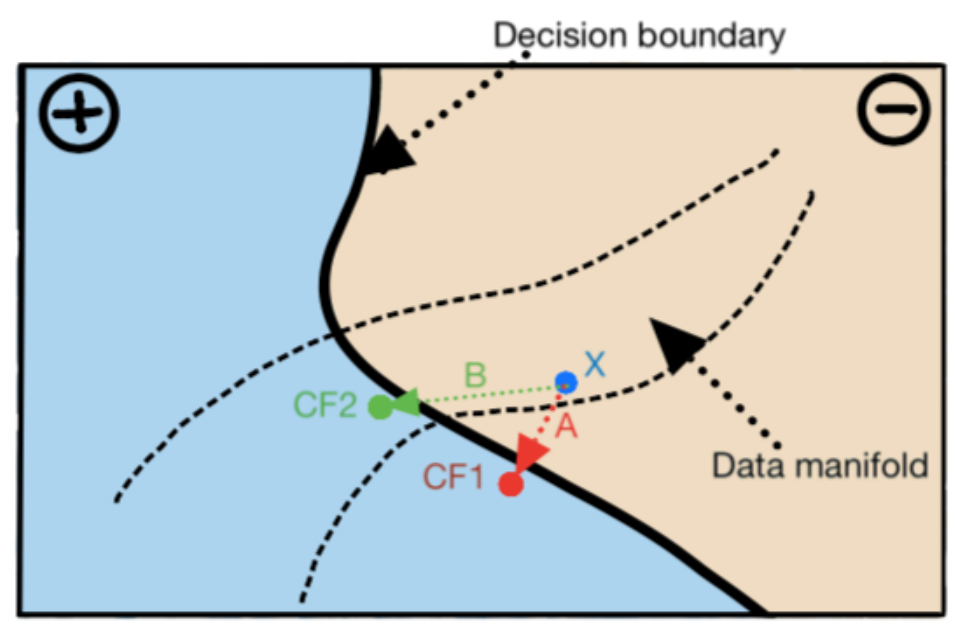
\includegraphics[width=1\textwidth]{figure/counterfactuals_obj}
		\end{center}
		
		\scriptsize{\textbf{Figure:} Two possible paths for a datapoint \textcolor{blue}{$\xv$},
			originally classified in the negative class. The two counterfactuals (\textcolor{red}{CF1} and \textcolor{green}{CF2}) are valid. Note that the red path $A$ for CF1 is the shortest, whereas the
			green path $B$ for CF2 adheres closely to the manifold of the training data, but is longer.}
		\vspace{0.3cm}
		
		\tiny{Source: Verma et al. (2020)}
		
		\vspace{0.3cm}
	\end{column}
	\end{columns}
	\begin{itemize}
		\item For example, $o_4$ could then be the Gower distance of $\xv'$ to the nearest data point of the training dataset $\xv^{[1]}$
	$$o_4(\xv', \Xmat) = \Gower(\xv', \xv^{[1]}) = \frac{1}{p} \sum_{j = 1}^{p}  \delta_G(x_j', x^{[1]}_j).$$
		\end{itemize}
	
	Overall, we could update Eq.~(\ref{eq:optim}) to be: 
	\begin{equation}
		\argmin_{\xv'} \lambda_1 o_1(\fh(\xv'), y') + \lambda_2 o_2(\xv', \xv) + \lambda_3 o_3(\xv', \xv) + \lambda_4 o_4(\xv', \Xmat).
	\end{equation}


\footnote[frame]{Verma et al. (2020). \href{https://arxiv.org/pdf/2010.10596.pdf}{Counterfactual Explanations for Machine Learning: A Review.}}

\end{vbframe}

\begin{vbframe}{Remarks: The Rashomon Effect}
The solution to the optimization problem might not be unique, there can be many equally close inputs that obtain the desired classification. Correspondingly, there can be many different equally good explanations for the same decision. This is called the \textbf{Rashomon effect}.
	\begin{itemize}
		\item We could present all CEs for a given case; however, time is limited and so is the human processing capacity.
		\item Another solution is to focus on one or few CEs; however, by which criterion should they be selected?
		\item Worse, as the model is generally non-linear, inconsistent CEs can arise e.g. suggesting either an increase or decrease in credit duration, which confuses the explainee.
		\item How to deal with the Rashomon effect is considered an open problem in IML.
	\end{itemize}
\end{vbframe}

\begin{vbframe}{Remarks: Model or Real-World}
Most CEs provide explanations of model-predictions. However, to end-users, these explanations appear to explain the process in which the model is employed. Unfortunately, the transfer from the model to the real-world is generally not permitted.
	\begin{itemize}
	\item Consider, e.g., a CE that proposes to increase the feature age by 5 to obtain the loan. A loan applicant takes this information and applies 5 years later for the loan. 
	\item However, by then, many of her properties have changed not only the age since they are causally dependent on age like income or the job status.
	%\item Also, the algorithm can change and CEs are not applicable anymore.
	%\item Even worse, the user might have typos in the application and in fact no changes are necessary to obtain the loan.
	\item Karimi et al. (2020) avoid this shortcoming by considering causal dependencies between variables.
%		\item Actionability: We could further strengthen above's plausibility criterion by requiring counterfactuals that do not change immutable features (e.g., race, city of birth, sex). Therefore, we could  search for counterfactuals only among a defined feasible set of counterfactuals $\mathcal{A}$. 
%		\item Causality: We could also restrict the search to counterfactuals that maintain any known causal relations. In the real world, if one feature is changed it affects also other features. E.g., better skills lead to better salary, but also a higher age due to the necessary training. 
	\end{itemize}
\footnote[frame]{Karimi et al. (2021). Algorithmic Recourse: From Counterfactual Explanations to Interventions.  Proceedings of the 2021 ACM Conference on Fairness, Accountability, and Transparency. 353–362.}
\end{vbframe}


\endlecture
\end{document}